\documentclass{standalone}
\usepackage{tikz}
\usetikzlibrary{patterns, positioning}

\begin{document}
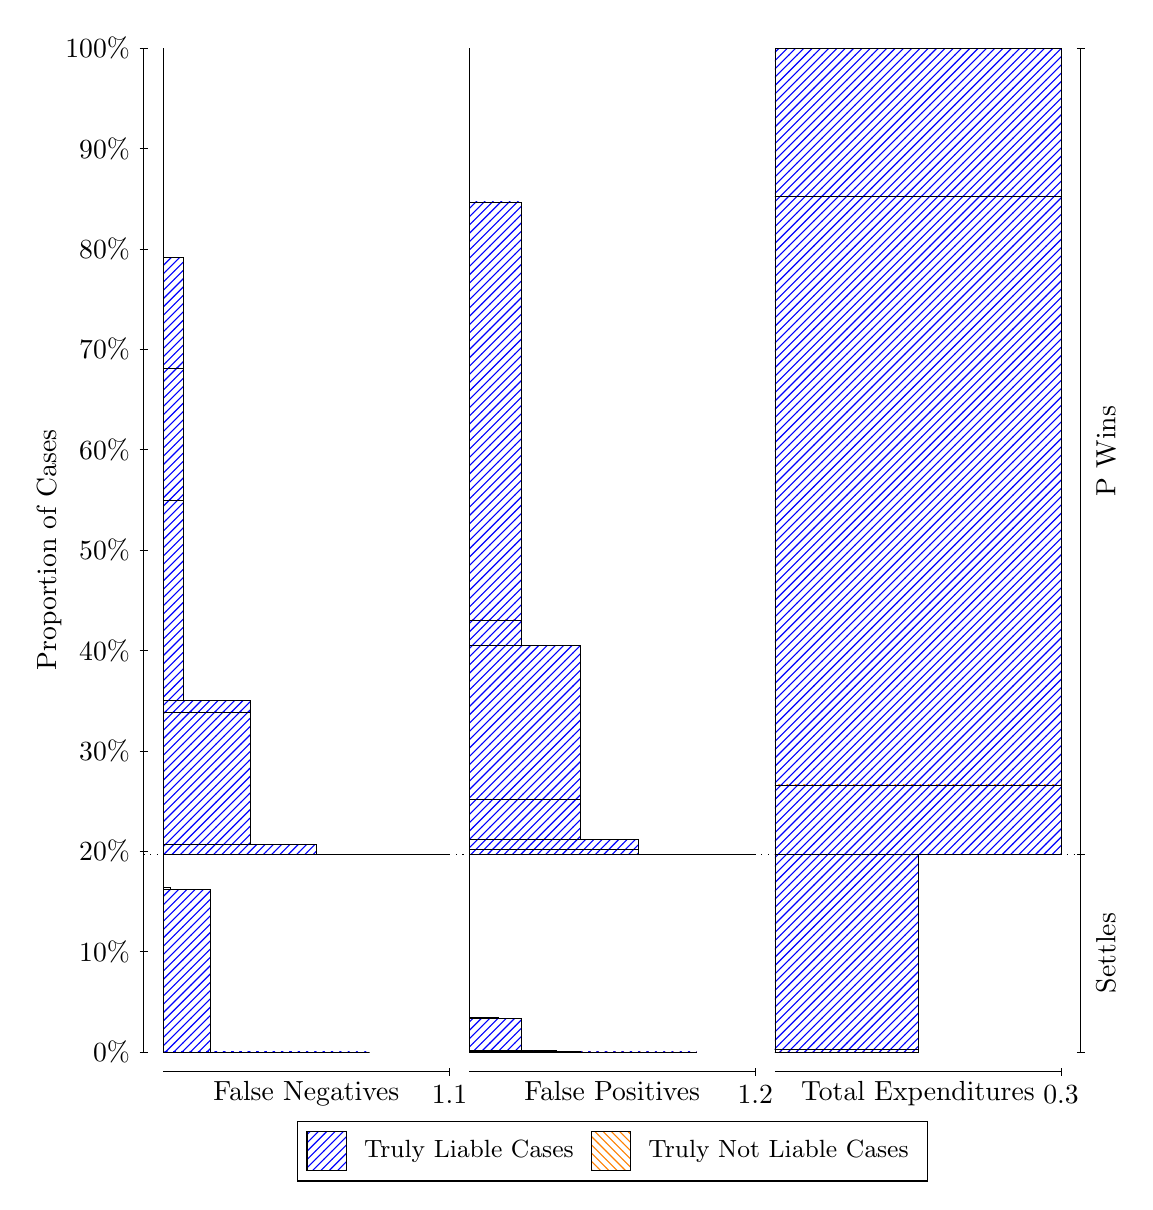
\begin{tikzpicture}
\draw[black, very thin] (1.5,1.75) -- (1.5,14.5);
\node[rotate=90, anchor=center] at (0.3, 8.125) {Proportion of Cases};
\draw[black, very thin] (1.45,1.75) -- (1.55,1.75);
\node[anchor=east] at (1.45, 1.75) {0\%};
\draw[black, very thin] (1.45,3.025) -- (1.55,3.025);
\node[anchor=east] at (1.45, 3.025) {10\%};
\draw[black, very thin] (1.45,4.3) -- (1.55,4.3);
\node[anchor=east] at (1.45, 4.3) {20\%};
\draw[black, very thin] (1.45,5.575) -- (1.55,5.575);
\node[anchor=east] at (1.45, 5.575) {30\%};
\draw[black, very thin] (1.45,6.85) -- (1.55,6.85);
\node[anchor=east] at (1.45, 6.85) {40\%};
\draw[black, very thin] (1.45,8.125) -- (1.55,8.125);
\node[anchor=east] at (1.45, 8.125) {50\%};
\draw[black, very thin] (1.45,9.4) -- (1.55,9.4);
\node[anchor=east] at (1.45, 9.4) {60\%};
\draw[black, very thin] (1.45,10.675) -- (1.55,10.675);
\node[anchor=east] at (1.45, 10.675) {70\%};
\draw[black, very thin] (1.45,11.95) -- (1.55,11.95);
\node[anchor=east] at (1.45, 11.95) {80\%};
\draw[black, very thin] (1.45,13.225) -- (1.55,13.225);
\node[anchor=east] at (1.45, 13.225) {90\%};
\draw[black, very thin] (1.45,14.5) -- (1.55,14.5);
\node[anchor=east] at (1.45, 14.5) {100\%};

\draw[black, very thin] (13.4,1.75) -- (13.4,14.5);
\draw[black, very thin] (13.35,1.75) -- (13.45,1.75);
\node[anchor=west] at (13.35, 1.75) {};
\draw[black, very thin] (13.35,4.2611) -- (13.45,4.2611);
\node[anchor=west] at (13.35, 4.2611) {};
\draw[black, very thin] (13.35,14.5) -- (13.45,14.5);
\node[anchor=west] at (13.35, 14.5) {};

\draw[black, very thin, pattern color=blue, pattern=north east lines] (1.75,1.75) rectangle (4.3694,1.75);
\draw[black, very thin, pattern color=blue, pattern=north east lines] (1.75,1.75) rectangle (4.0314,1.75);
\draw[black, very thin, pattern color=blue, pattern=north east lines] (1.75,1.75) rectangle (3.6934,1.75);
\draw[black, very thin, pattern color=blue, pattern=north east lines] (1.75,1.75) rectangle (3.5244,1.75);
\draw[black, very thin, pattern color=blue, pattern=north east lines] (1.75,1.75) rectangle (3.3554,1.75);
\draw[black, very thin, pattern color=blue, pattern=north east lines] (1.75,1.75) rectangle (3.1864,1.75);
\draw[black, very thin, pattern color=blue, pattern=north east lines] (1.75,1.75) rectangle (3.0174,1.75);
\draw[black, very thin, pattern color=blue, pattern=north east lines] (1.75,1.75) rectangle (2.8484,1.75);
\draw[black, very thin, pattern color=blue, pattern=north east lines] (1.75,1.75) rectangle (2.6795,1.7502);
\draw[black, very thin, pattern color=blue, pattern=north east lines] (1.75,1.7502) rectangle (2.5105,1.7502);
\draw[black, very thin, pattern color=blue, pattern=north east lines] (1.75,1.7502) rectangle (2.3415,1.7503);
\draw[black, very thin, pattern color=blue, pattern=north east lines] (1.75,1.7503) rectangle (2.3415,3.8193);
\draw[black, very thin, pattern color=blue, pattern=north east lines] (1.75,3.8193) rectangle (2.1725,3.8193);
\draw[black, very thin, pattern color=blue, pattern=north east lines] (1.75,3.8193) rectangle (2.0035,3.8194);
\draw[black, very thin, pattern color=blue, pattern=north east lines] (1.75,3.8194) rectangle (1.8345,3.8363);
\draw[black, very thin, pattern color=orange, pattern=north west lines] (1.75,3.8363) rectangle (1.75,3.8363);
\draw[black, very thin, pattern color=blue, pattern=north east lines] (1.75,3.8363) rectangle (1.75,4.2611);
\draw[black, very thin, pattern color=blue, pattern=north east lines] (1.75,4.2611) rectangle (5.3833,4.2611);
\draw[black, very thin, pattern color=blue, pattern=north east lines] (1.75,4.2611) rectangle (4.5384,4.2623);
\draw[black, very thin, pattern color=blue, pattern=north east lines] (1.75,4.2623) rectangle (3.6934,4.3826);
\draw[black, very thin, pattern color=blue, pattern=north east lines] (1.75,4.3826) rectangle (2.8484,6.0686);
\draw[black, very thin, pattern color=blue, pattern=north east lines] (1.75,6.0686) rectangle (2.8484,6.2164);
\draw[black, very thin, pattern color=blue, pattern=north east lines] (1.75,6.2164) rectangle (2.0035,8.761);
\draw[black, very thin, pattern color=blue, pattern=north east lines] (1.75,8.761) rectangle (2.0035,10.437);
\draw[black, very thin, pattern color=blue, pattern=north east lines] (1.75,10.437) rectangle (2.0035,11.843);
\draw[black, very thin, pattern color=orange, pattern=north west lines] (1.75,11.843) rectangle (1.75,11.843);
\draw[black, very thin, pattern color=blue, pattern=north east lines] (1.75,11.843) rectangle (1.75,14.5);
\draw[black, very thin, pattern color=orange, pattern=north west lines] (5.6333,1.75) rectangle (8.5252,1.75);
\draw[black, very thin, pattern color=blue, pattern=north east lines] (5.6333,1.75) rectangle (8.5252,1.75);
\draw[black, very thin, pattern color=orange, pattern=north west lines] (5.6333,1.75) rectangle (7.932,1.75);
\draw[black, very thin, pattern color=blue, pattern=north east lines] (5.6333,1.75) rectangle (7.932,1.75);
\draw[black, very thin, pattern color=blue, pattern=north east lines] (5.6333,1.75) rectangle (7.7837,1.75);
\draw[black, very thin, pattern color=orange, pattern=north west lines] (5.6333,1.75) rectangle (7.6354,1.75);
\draw[black, very thin, pattern color=blue, pattern=north east lines] (5.6333,1.75) rectangle (7.6354,1.75);
\draw[black, very thin, pattern color=orange, pattern=north west lines] (5.6333,1.75) rectangle (7.3388,1.75);
\draw[black, very thin, pattern color=blue, pattern=north east lines] (5.6333,1.75) rectangle (7.3388,1.75);
\draw[black, very thin, pattern color=blue, pattern=north east lines] (5.6333,1.75) rectangle (7.1905,1.75);
\draw[black, very thin, pattern color=orange, pattern=north west lines] (5.6333,1.75) rectangle (7.0422,1.75);
\draw[black, very thin, pattern color=blue, pattern=north east lines] (5.6333,1.75) rectangle (7.0422,1.75);
\draw[black, very thin, pattern color=blue, pattern=north east lines] (5.6333,1.75) rectangle (7.0422,1.7534);
\draw[black, very thin, pattern color=blue, pattern=north east lines] (5.6333,1.7534) rectangle (6.8939,1.7534);
\draw[black, very thin, pattern color=orange, pattern=north west lines] (5.6333,1.7534) rectangle (6.7456,1.7534);
\draw[black, very thin, pattern color=blue, pattern=north east lines] (5.6333,1.7534) rectangle (6.7456,1.7729);
\draw[black, very thin, pattern color=blue, pattern=north east lines] (5.6333,1.7729) rectangle (6.5973,1.773);
\draw[black, very thin, pattern color=blue, pattern=north east lines] (5.6333,1.773) rectangle (6.449,1.773);
\draw[black, very thin, pattern color=blue, pattern=north east lines] (5.6333,1.773) rectangle (6.3007,1.773);
\draw[black, very thin, pattern color=blue, pattern=north east lines] (5.6333,1.773) rectangle (6.3007,2.1747);
\draw[black, very thin, pattern color=blue, pattern=north east lines] (5.6333,2.1747) rectangle (6.1524,2.1747);
\draw[black, very thin, pattern color=blue, pattern=north east lines] (5.6333,2.1747) rectangle (6.0041,2.1917);
\draw[black, very thin, pattern color=blue, pattern=north east lines] (5.6333,2.1917) rectangle (5.8558,2.1917);
\draw[black, very thin, pattern color=blue, pattern=north east lines] (5.6333,2.1917) rectangle (5.7075,2.1917);
\draw[black, very thin, pattern color=blue, pattern=north east lines] (5.6333,2.1917) rectangle (5.6333,4.2611);
\draw[black, very thin, pattern color=orange, pattern=north west lines] (5.6333,4.2611) rectangle (9.2667,4.2611);
\draw[black, very thin, pattern color=blue, pattern=north east lines] (5.6333,4.2611) rectangle (9.2667,4.2611);
\draw[black, very thin, pattern color=blue, pattern=north east lines] (5.6333,4.2611) rectangle (8.5252,4.2622);
\draw[black, very thin, pattern color=orange, pattern=north west lines] (5.6333,4.2622) rectangle (8.5252,4.2622);
\draw[black, very thin, pattern color=blue, pattern=north east lines] (5.6333,4.2622) rectangle (8.5252,4.2636);
\draw[black, very thin, pattern color=blue, pattern=north east lines] (5.6333,4.2636) rectangle (7.7837,4.3205);
\draw[black, very thin, pattern color=orange, pattern=north west lines] (5.6333,4.3205) rectangle (7.7837,4.3205);
\draw[black, very thin, pattern color=blue, pattern=north east lines] (5.6333,4.3205) rectangle (7.7837,4.4539);
\draw[black, very thin, pattern color=blue, pattern=north east lines] (5.6333,4.4539) rectangle (7.0422,4.959);
\draw[black, very thin, pattern color=orange, pattern=north west lines] (5.6333,4.959) rectangle (7.0422,4.959);
\draw[black, very thin, pattern color=blue, pattern=north east lines] (5.6333,4.959) rectangle (7.0422,6.9177);
\draw[black, very thin, pattern color=blue, pattern=north east lines] (5.6333,6.9177) rectangle (6.3007,7.2361);
\draw[black, very thin, pattern color=orange, pattern=north west lines] (5.6333,7.2361) rectangle (6.3007,7.2361);
\draw[black, very thin, pattern color=blue, pattern=north east lines] (5.6333,7.2361) rectangle (6.3007,12.545);
\draw[black, very thin, pattern color=blue, pattern=north east lines] (5.6333,12.545) rectangle (5.6333,14.5);
\draw[black, very thin, pattern color=orange, pattern=north west lines] (9.5167,1.75) rectangle (11.333,1.75);
\draw[black, very thin, pattern color=blue, pattern=north east lines] (9.5167,1.75) rectangle (11.333,1.7867);
\draw[black, very thin, pattern color=orange, pattern=north west lines] (9.5167,1.7867) rectangle (11.333,1.7867);
\draw[black, very thin, pattern color=blue, pattern=north east lines] (9.5167,1.7867) rectangle (11.333,1.7868);
\draw[black, very thin, pattern color=orange, pattern=north west lines] (9.5167,1.7868) rectangle (11.333,1.7868);
\draw[black, very thin, pattern color=blue, pattern=north east lines] (9.5167,1.7868) rectangle (11.333,4.2611);
\draw[black, very thin, pattern color=orange, pattern=north west lines] (9.5167,4.2611) rectangle (13.15,4.2611);
\draw[black, very thin, pattern color=blue, pattern=north east lines] (9.5167,4.2611) rectangle (13.15,5.1425);
\draw[black, very thin, pattern color=orange, pattern=north west lines] (9.5167,5.1425) rectangle (13.15,5.1425);
\draw[black, very thin, pattern color=blue, pattern=north east lines] (9.5167,5.1425) rectangle (13.15,12.619);
\draw[black, very thin, pattern color=orange, pattern=north west lines] (9.5167,12.619) rectangle (13.15,12.619);
\draw[black, very thin, pattern color=blue, pattern=north east lines] (9.5167,12.619) rectangle (13.15,14.5);
\draw[black, dotted] (1.5,4.2611) -- (13.4,4.2611);
\draw[black, very thin] (1.75,1.5) -- (5.3833,1.5);
\node[anchor=north] at (3.5667, 1.5) {False Negatives};
\draw[black, very thin] (5.3833,1.45) -- (5.3833,1.55);
\node[anchor=north] at (5.3833, 1.45) {1.1};

\draw[black, very thin] (5.6333,1.5) -- (9.2667,1.5);
\node[anchor=north] at (7.45, 1.5) {False Positives};
\draw[black, very thin] (9.2667,1.45) -- (9.2667,1.55);
\node[anchor=north] at (9.2667, 1.45) {1.2};

\draw[black, very thin] (9.5167,1.5) -- (13.15,1.5);
\node[anchor=north] at (11.333, 1.5) {Total Expenditures};
\draw[black, very thin] (13.15,1.45) -- (13.15,1.55);
\node[anchor=north] at (13.15, 1.45) {0.3};

\node[black, centered, rotate=90] at (13.72, 3.0055) {Settles};
\node[black, centered, rotate=90] at (13.72, 9.3805) {P Wins};

\draw (7.449999999999999,1.5) node[draw=none] (baseCoordinate) {};
\begin{scope}[align=center]
        \matrix[scale=0.5, draw=black, below=0.5cm of baseCoordinate, nodes={draw}, column sep=0.1cm]{
            \node[rectangle, draw, minimum width=0.5cm, minimum height=0.5cm, pattern=north east lines, pattern color=blue] {}; &
            \node[draw=none, font=\small] (B) {Truly Liable Cases}; &
            \node[rectangle, draw, minimum width=0.5cm, minimum height=0.5cm, pattern=north west lines, pattern color=orange] {}; &
            \node[draw=none, font=\small] (B) {Truly Not Liable Cases}; \\
            };
\end{scope}

\end{tikzpicture}
\end{document}